\documentclass[../ala_hataile.tex]{subfiles}
\begin{document}

\includepdf[pages=10-11, pagecommand={}]{sisasivut_19062018.pdf}
\twocolumn[\section{Tähtitiede}]
\subsection*{Yleistä}
Helsingin observatoriolta Kumpulan
Physicumiin vuonna 2010 muuttanut
tähtitiede majailee nykyään
kolmannen kerroksen keskikäytävällä
Fysiikan osastolla
yhdessä hiukkasfyysikoiden ja kosmologien
kanssa.

\begin{figure*}[b!]
	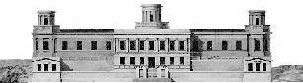
\includegraphics[width=\textwidth]{tahtitieteenlaitos.png}
\end{figure*}

Viime vuosina valmistuneet tähtitieteilijät
ovat työllistyneet pääasiassa tutkimusja
opetustehtäviin yliopistoihin, muihin
tutkimuslaitoksiin tai yritysmaailmaan.
Ammattitähtitieteilijän tehtävät vaativat
tohtorin tutkintoa ja lähes kaikki tähtitieteestä
maisteriksi valmistuvat jatkavat
opintojaan väitöskirjaan asti, joko Helsingissä
tai ulkomailla. Helsingissä tähtitieteen
tohtorinkoulutuksesta vastaa Alkeishiukkasfysiikan
ja maailmankaikkeuden
tutkimuksen tohtoriohjelma PAPU.

\subsection*{Tähtitiede sivutieteenalana}
Tähtitiede on osana luonnontieteellistä
perussivistystä hyödyllinen sivutieteenala kaikille,
etenkin fysikaalisten tieteiden opiskelijoille
ja opettajankoulutuslinjalaisille.
Tähtitiede on myös hyvin joustava tieteenala,
sillä sen voi suorittaa 15 tai 25~op laajuisena, ja sivutieteenalaopiskelijoille ainoat pakolliset
kurssit ovat TäPe~I ja II.
\subsection*{Tähtitiedettä kaikille}
Pari kertaa vuodessa luennoitava Maailmankaikkeus
Nyt! "-kurssi on yksi yliopiston
suosituimpia kursseja. Se käsittelee
tähtitieteen perusasiat ilman matematiikkaa
ja soveltuu erinomaisesti kaikille yleissivistyksen
parantamiseksi. Kurssin ruotsinkielisellä
versiolla on mahdollista suorittaa
pakolliset ruotsin opinnot ja kurssi luennoidaan
myös englanniksi.
\subsection*{Astrofysiikan perusteet}
Tähtitieteen perusopinnoissa tutustutaan
pintapuolisesti kaikkiin tähtitieteen osa-alueisiin.
Tämän lisäksi opetellaan perusteellisesti
tähtitieteen peruskäsitteet ja havaintomenetelmät.
Perusopinnot eivät ole matemaattisesti haastavia, vaikka asioiden
matemaattisempi käsittely voi olla uusi asia
myös tähtitiedettä pidempään harrastaneelle.

\subsubsection*{Tähtitieteen perusteet~I ja II (5+5~op)}
Tähtitieteen perusteilla opitaan perusasiat
tähtitieteellisistä kohteista, metodeista
ja havaintovälineistä. Tutuksi tulevat niin
pallomaiset tähtijoukot, magnitudit kuin
spektroskopiakin. Kolmannessa periodissa
alkavalla TäPe~I:llä opetellaan ensin
perusasiat koordinaatistoista, havaintolaitteista
ja fotometrisistä käsitteistä. Kurssin
loppupuolella tulevat tutuksi säteilymekanismit,
taivaankappaleiden liikkeet ja ensimmäinen
tähtitieteellinen kohde, Aurinkokunta.
Neljännellä periodilla alkaa TäPe~II, jolla
keskitytään erilaisiin tähtitieteellisiin kohteisiin.
Tähdistä ja tähtienvälisestä aineesta
siirrytään galaksien kautta maailmankaikkeuden
suuren mittakaavaan rakenteisiin.
Kurssiin lopulla tutustutaan lyhyesti myös
astrobiologiaan, eli maapallon ulkopuolella
esiintyvän elämän olemassaolon edellytyksiin.

\subsubsection*{Johdatus avaruusplasmafysiikkaan (5~op)}
Kurssilla tutustutaan plasman perusominaisuuksiin, 
erilaisten plasmojen käytökseen sekä magneettikentän 
vaikutukseen. Kohteita ovat myös plasman käytös auringossa, 
sekä fuusio sekä maan päällä että avaruudessa. 

\subsubsection*{Havaitsevan tähtitieteen peruskurssi~I (5~op)}
Hava~I:llä tutustutaan perusteellisesti
tähtitieteellisten havaintojen tekoon. Kurssilla
käsitellään optista, eli näkyvän valon,
tähtitiedettä, mutta perusperiaatteet pätevät
myös muilla aallonpituusalueilla. Kurssilla
opitaan mm.\,miten havaintolaitteet, esim.\,CCD-kamerat toimivat ja millaisia eri havaintomenetelmiä
on käytössä. Kurssilla
on myös perinteisesti tehty vierailu Kirkkonummella
sijaitsevaan Metsähoviin, jossa
on yliopiston oma 60-senttinen kaukoputki.
\subsubsection*{Havaitsevan tähtitieteen peruskurssi~II (5~op)}
Kolmoisperiodille ajoittuvalla
Hava~II:lla laajennetaan havaintoja optisen
alueen ulkopuolelle, radio-, röntgen- ja
gammatähtitieteeseen. Menetelmien lisäksi
kurssilla opitaan mitä haasteita ja mahdollisuuksia
eri aallonpituusalueet tuovat mukanaan. 

\subsection*{Teoreettinen astrofysiikka}
Perusopintojen osittain pintapuolisen
käsittelyn jälkeen aineopinnoissa tutustutaan
tähtitieteen eri osa-alueisiin tarkemmin, kunkin kurssin keskittyessä yhteen
osa-alueeseen. Jotkin aineopintojen kurssit
kuuluvat vaativimpiin kursseihin koko tähtitieteessä,
mutta niiden asiat ovat välttämättömiä
tähtitieteen syvällisen osaamisen
kannalta. Aineopintojen jälkeen opiskelijalla
on vankka pohja lähteä keskittymään
mihin tahansa tähtitieteen suuntaukseen.

\subsubsection*{Astrofysiikan peruskurssi~I--II (5+5~op)}
Tähtitiedettä teoreettisimmillaan. Säteilynkuljetuksen,
termofysiikan ja Planckin,
Maxwellin, Boltzmannin, Eddingtonin
sekä Sahan teorioiden avulla pyritään ymmärtämään
tähtien rakennetta, atmosfääriä,
tähtienvälistä ainetta ja spektriviivojen
syntyä. Työläs, mutta kaiken tähtitieteen
kannalta hyödyllinen (ellei jopa välttämätön)
kurssi.

\subsubsection*{Taivaanmekaniikan peruskurssi~I--II (5+5~op)}
Kahden ja kolmen kappaleen ongelmat
Newtonin, Lagrangen ja Hamiltonin mekaniikan
avulla. Kurssin testilaboratoriona
toimii Aurinkokunta. Yksittäiset laskaritehtävät
kuten Gaussin radanmääritys ovat
tähtitieteen pisimpiä. Normaalien laskareiden ja tentin lisäksi kurssiin sisältyy harjoitustyö.
\subsection*{Astrofysiikan kohteet}
\subsubsection*{Aurinkokunnan fysiikka (5~op)}
Kurssin aiheena on planeettojen ja aurinkokunnan
pienkappaleiden fysiikka ja
tärkeimpinä menetelminä säteilynkuljetus
ja fotometria. Itsenäistä tiedonhankintaa ja
esittämistä harjoitellaan pitämällä esitelmä
jostakin kurssin aiheesta.
\begin{figure}[b]
	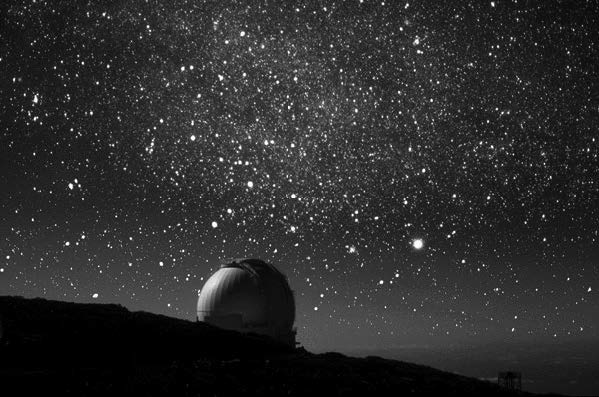
\includegraphics[width=\columnwidth]{not.png}
\end{figure}
\subsubsection*{Galaksit ja kosmologia (5~op)}
Kurssin aiheena on galaksien rakenne,
synty ja kehitys, sekä kosmologia tähtitieteilijälle
ystävällisessä muodossa. Niin galaksityypit,
kotoisa galaksiryhmämme kuin
maailmankaikkeuden suuren mittakaavan
rakenne tulevat tutuksi. Kurssilla tutustutaan
myös universumin kehitystä kuvaaviin
Friedmannin yhtälöihin. VAROITUS!
Kurssilla voit törmätä myös mustiin aukkoihin,
kvasaareihin, pimeään aineeseen ja
pimeään energiaan.
\subsubsection*{Linnunradan rakenne (5~op)}
Kurssilla tutustutaan lähemmin kotigalaksiimme,
Linnunrataan. Siellä opitaan
millainen rakenne Linnunradalla on ja miten
sitä voidaan tutkia.

\begin{figure}
	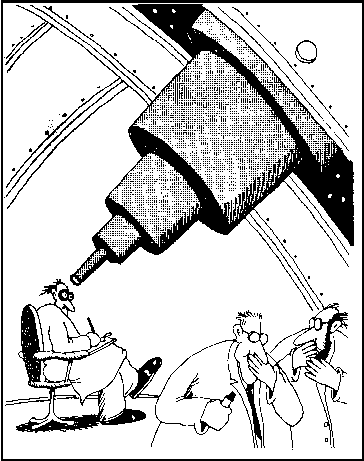
\includegraphics[width=\columnwidth]{teleskooppi.png}
\end{figure}
\subsubsection*{Tähtien rakenne ja kehitys (5~op)}
Vaikka tähtimallien laskeminen on supertietokoneiden
työtä, voi sopivilla yksinkertaisilla
malleilla saada tietoa tähtien kehityksestä
pelkällä kynällä ja paperillakin.
Kurssi alkaa tähtien rakenteen perusyhtälöiden
johtamisesta, jonka jälkeen käydään
läpi tähtien kehityskaari molekyylipilvestä
kompaktiin tähtijäänteeseen.

\subsection*{Maisteriohjelman maistelukursseja}
\subsubsection*{Plasma Physics (5~op)}
Maisteriopintojen yksi pakollinen kurssi, joka jatkaa johdatus avaruusplasmafysiikan aiheita. Kurssilla oletetaan hyvä elektrodynamiikan tuntemus. Kurssilla tutustutaan plasman ominaisuuksiin, magnetohydrodynamiikkaan sekä fuusiotutkimukseen. Kurssi luennoidaan joka syksy, ja kuten kaikki maisterikurssit pääsääntöinen opetus ja materiaalit ovat englanniksi. 
\subsubsection*{Open Problems in Modern Astrophysics (5~op)}
Maisterivaiheen yksi kehutuimmasta kursseista. Kurssi keskittyy tämän ajan tähtiteteen kiinnostavimpiin ongelmiin. Aiheet vaihtuvat vuosittain, mutta aiempia aiheita ovat olleet mm. ruskeat kääpiötähdet, gamma\-säde\-purkaukset ja neutronitähdet, sekä eksoplaneetat. Kurssi suoritetaan lukemalla tieteellisiä artikkeleita aiheesta, ja siten opiskelija saa kokemusta tieteellisen tekstin lukemisesta. Kurssi soveltuu hyvin toisen tai kolmannen vuoden opintoihin.

\vspace{0.5cm}
\noindent
\textsc{Jussi Aaltonen}\\
\textsc{Antti Rantala}\\
\textsc{Antton Luoma}\\
\textsc{Emma Mannfors}

\end{document}